%version of 06-05-18
\documentclass{article}
\usepackage{amsfonts,amsmath,amsthm,amssymb,fullpage,makeidx,epsfig}
\usepackage{mathptmx}
\usepackage{amssymb}
\usepackage{helvet}
\usepackage{courier}
\usepackage{makeidx}
\usepackage{graphicx}
\usepackage{multicol}
\usepackage{epsfig}
\input preamble

\begin{document}

\begin{center}
{\bf SUMMATION}
\end{center}

%\chapter{SUMMATION}
%\label{ch:Summation}

\section{Manifesto}


\subsection{The Goal of This Chapter}


The fundamental goal of this book / chapter / section is to endow the
reader with an operational level of conceptual and methodological
understanding of the discrete mathematics that is used to study and
understand computing.  We construe an ``operational'' level of
understanding to be one that enables the reader to ``do'' mathematics.

Somewhat surprising to the non-mathematician, a large portion of
``doing'' mathematics, the widely touted ``queen of the sciences'', is
pattern-matching---albeit of a monumentally sophisticated variety.
Mathematicians are trained to understand pieces of reality to a depth
that allows them to understand how apparently unrelated concepts $A$
and $B$ can be conceptualized via the same abstract representation,
and to analyze (computational, in our bailiwick) advantages to
exploiting such representations.

Toward the end of guiding the reader through this forest of
abstractions, we categorize our targets in three ways
\begin{enumerate}
\item
fundamental sums

of intrinsic intererest

e.g.: arithmetic sums, geometric sums, mathematically ``smooth'' sums

\item
fundamental techniques

that work in many distinct situations

e.g.: using integration for summation; grouping/replication; verification via induction

\item
fundamental representations

that enable one to study the same phenomenon in many seemingly unrelated ways

e.g.: numbers, Riemann sums, slices of pie, tokens arranged in stylized ways
\end{enumerate}


\section{Introduction}
\label{sec:intro}

The operation of {\it summation}---adding up aggregates of
numbers---is of fundamental importance in the world of digital
computing.  While we humans are able to deal handily with abstractions
such as ``smoothness'' and ``continuity'', we must employ
sophisticated {\em discretizations} of these concepts in order to
enlist the aid of digital computers in dealing with such abstractions.
Summations provide a very useful discretization of ``continuous'' or
``smooth'' phenomena that are typically dealt with by humans with the
aid of the calculus that was invented by Newton and Leibnitz for such
dealings.

This chapter is dedicated to exploring how to employ summations as a
computational tool.  We deal throughout with {\it series}, i.e.,
(possibly infinite) sequences of numbers
\[ a_1, a_2, \ldots \]
whose sum
\[ a_1 + a_2 + \cdots \]
is of interest.

As a simple illustration, consider the following puzzle.  You are
presented with a traditional $8 \times 8$ chess board, plus an offer
of a one-time gift of {\em one million euros}.  In place of this
one-time gift, you can opt for the money amassed in the following
way.

\noindent
%
I will go along the chessboard row by row.  I will place $1$ euro in
the first square I encounter, $4 \ (= 2^2)$ euros in the second, $9
\ (= 3^2)$ euros in the third , \ldots, $4096 \ (= 64^2)$ euros in the
last square.

\noindent
{\em WHICH CHOICE DO YOU MAKE?}

\medskip

By the end of this chapter, you will be able to determine in minutes
that the {\em alternative} offer (the one that uses the chessboard)
would net you a sum of 8,390,656 euros---clearly the preferable
choice!



\section{Summing Structured Series}
\label{sec:structured-series}

\subsection{Arithmetic Sums and Series}
\label{sec:arithmetic-series}

We define arithmetic sequences and learn how to calculate their sums.

\begin{equation}
\label{eq:arith-seq}
\begin{array}{l}
\mbox{An $n$-term arithmetic sequence:} \\
\hspace*{.25in}a, \ a+b, \ a+2b, \ a+3b, \ \ldots, a+(n-1)b \\
\\
\mbox{The corresponding arithmetic series:} \\
\hspace*{.25in}a + (a+b) + (a+2b) + (a+3b) + \cdots + (a+(n-1)b) \\
\hspace*{.5in} = \
an + b \cdot (1 + 2 + \cdots + n-1)
\end{array}
\end{equation}
We can, thus, sum the arithmetic series in (\ref{eq:arith-seq}) by
determining the sum of the first $m$ positive integers; $m = n-1$ in
(\ref{eq:arith-seq}).  We use this result as an opportubnity to
introduce important notation.

%\addcontentsline{toc}{paragraph}{-- A fun result: Summing the first
%  $n$ integers}

\noindent {\bf Proposition}
\label{thm:sum-first-integers-Gauss}
For all $n \in \N$,
\begin{eqnarray}
\nonumber
S_1(n) \ \eqdef \ \sum_{i=1}^n \ i
  & \eqdef &
 1 + 2 + \cdots + (n-1) + n \\
\label{eq:sum-1-to-n}
  & = & \frac{1}{2} n (n+1) \\
\nonumber
  & = & {{n+1}  \choose 2}.
\end{eqnarray}

\begin{proof}
The {\em constructive} proof\footnote{The proof is {\em constructive}
  in that it actually derives an answer.  This is in contrast to, say,
  the inductive proof of Proposition~\ref{thm:sum-1-to-n-induction},
  which just verifies a ``guessed'' answer.}~of summation
(\ref{eq:sum-1-to-n}) that we present now employs a device known to
the eminent German mathematician Karl Friedrich Gauss \index{Gauss,
  Karl Friedrich} as a pre-teenager.
\begin{equation}
\label{eq:arith-series}
\begin{array}{llccccccccc}
\mbox{Write $S_1(n)$ ``forwards'':} &
\hspace*{.25in}\sum_{i=1}^n \ = & 1 & + & 2   & + & \cdots & + & (n-1) & + & n \\
 & & & & & & & & & &  \\
\mbox{Write $S_1(n)$ ``in reverse'':} &
\hspace*{.25in}\sum_{i=1}^n \ = & n & + & (n-1) & + & \cdots & + & 2   & + & 1
\end{array}
\end{equation}
Now add the two representations of $S_1(n)$ in (\ref{eq:arith-series})
{\em columnwise}.  Because each of the $n$ column-sums equals $n+1$,
we find that $2 S_1(n) = n(n+1)$, which we easily rewrite as in
(\ref{eq:sum-1-to-n}) (after multiplying both sides of the equation by
$2$).  \qed
\end{proof}

It follows that our original series in (\ref{eq:arith-seq}) sums as
follows.
\[
a + (a+b) + (a+2b) + (a+3b) + \cdots + (a+(n-1)b) \ = \
an + b \cdot {n \choose 2}. 
\]

\medskip

We can build on Proposition~\ref{thm:sum-first-integers-Gauss} to
craft {\em two} ``constructive'' proofs---i.e., proof that explicitly
calculate the summation---that each perfect square, say, $m^2$, is the
sum of the first $m$ odd integers, $1, 3, 5, \ldots, 2m-1$.  These
proofs complement the ``guess-and-verify'' inductive proof of the same
result in Proposition~\ref{thm:squares-odd-integers-induction}.

%\addcontentsline{toc}{paragraph}{-- A fun result: The $n$th perfect
%  square is the sum of the first $n$ odd integers (two proofs)}

\noindent {\bf Proposition}
\label{thm:squares-odd-integers-Gauss}
For all $n \in \N^+$,
\begin{equation}
\label{eq:sum-of-odds}
\sum_{k=1}^n \ (2k-1)
 \ = \ 1 + 3 + 5 + \cdots + (2n-1) \ = \ n^2.
\end{equation}
That, is, the $n$th perfect square is the sum of the first $n$ odd
integers.


Before presenting our two proofs of this result, we note that the
notation in (\ref{eq:sum-of-odds}) is perfectly general: every positive
odd integer $m$ can be written in the form $2n-1$ for some positive
integer $n$.

\smallskip

\begin{proof}
({\it Argument \#1}.)
%
By direct calculation, we have
\begin{eqnarray*}
\sum_{k=1}^n \ \left( 2k-1 \right)
   & = & 2 \sum_{k=1}^n \ k \ \ - \ n \\
   & = & 2 \frac{n (n+1)}{2} \ \ - \ n \ \ \ \ \mbox{ by
  Proposition~\ref{thm:sum-first-integers-Gauss}} \\
   & = & (n^2 + n) - n \\
   & = & n^2. \hfill \qed
\end{eqnarray*}
\end{proof}

\medskip

\begin{proof}
({\it Argument \#2}.)
%
Let us adapt Gauss's ``trick'' to this problem.  Let us denote the
target sum $\sum_{k=1}^n \ (2k-1)$ by $S(n)$. 
\begin{equation}
\label{eq:add-odds}
\begin{array}{llccccccccc}
\mbox{$S_n$ ``forwards'':} &
S(n) \ = 
& 1 & + & 3 & + & \cdots & + & (2n-3) & + & (2n-1) \\
 & & & & & & & & & &  \\
\mbox{$S_n$ ``in reverse'':} &
S(n) \ =
& (2n-1) & + & (2n-3) & + & \cdots & + & 3 & + & 1
\end{array}
\end{equation}
Now add the two representations of $S(n)$ in (\ref{eq:add-odds}) {\em
  columnwise}.  Because each of the $n$ column-sums equals $2n$, we
find that
\begin{equation}
\label{eq:sum-of-odds-sum}
2 S(n) \ = \ 2 \sum_{k=1}^n \ (2k-1) \ = \ 2n^2.
\end{equation}
We thus derive the desired summation (\ref{eq:sum-of-odds}) when we
divide both sides of equation (\ref{eq:sum-of-odds-sum}) by $2$.  \qed
\end{proof}

\subsection{Geometric Sums and Series}
\label{sec:geometric-sums}

We define geometric sequences and learn how to calculate their sums.

\begin{equation}
\label{eq:geom-seq}
\begin{array}{l}
\mbox{An $n$-term geometric sequence:} \\
\hspace*{.25in}a, \ ab, \ ab^2, \ \ldots, ab^{n-1} \\
\\
\mbox{The corresponding geometric series:} \\
\hspace*{.25in}a + ab + ab^2 + \cdots + ab^{n-1} \ = \
 a (1+ b + b^2 + \cdots + b^{n-1})
\end{array}
\end{equation}
It is clear just from this definition that we can sum the series in
(\ref{eq:geom-seq}) by summing just the sub-series
\begin{equation}
\label{eq:geom-series}
S_{b}(n) \ \eqdef \
1+ b + b^2 + \cdots + b^{n-1}.
\end{equation}

As we dvelop a solution technique for sub-series
(\ref{eq:geom-series}), we remark that when $b < 1$, an even simpler
solution technique

Toward the end of calculating the desired sum, we note the 



We proceed as follows.  Write $S_{b}(n)$ so that its terms are in {\em
  decreasing} order.  We thereby isolate two cases.
\begin{enumerate}
\item
Say first that $b > 1$.  In this case, we write the series in the form
\[ S^{b>1}_{b}(n) \ = \ b^{n-1} + b^{n-2} + \cdots + b^2 + b + 1, \]
and we note that
\[ S^{b>1}_{b}(n) \ = \
b^{n-1} \ + \ \frac{1}{b} \cdot S^{b>1}_{b}(n) \ - \ \frac{1}{b}. \]
In other words, we have
\[ \left( 1 - \frac{1}{b} \right)  S^{b>1}_{b}(n) \ = \ b^{n-1} -
\frac{1}{b}, \]
or equivalently,
\begin{equation}
\label{eq:geom-sum:b>1}
S^{b>1}_{b}(n) \ = \ \frac{b^{n}- 1}{b - 1}.
\end{equation}

\item
Alternatively, if $b < 1$, then we write the series in the form
\[ S^{b<1}_{b}(n) \ = \ 1+ b + b^2 + b^3 + \cdots + b^{n-1}. \]
and we note that
\[ S^{b<1}_{b}(n) \ = \
1 \ + \ b \cdot S^{b<1}_{b}(n) \ - \ b^n. \] 
In other words,
\[ (1-b) S^{b<1}_{b}(n) \ = \ 1 \ - \ b^n \]
or equivalently,
\begin{equation}
\label{eq:geom-sum:b<1}
S^{b<1}_{b}(n) \ = \ \frac{1 - b^n}{1-b}.
\end{equation}
\end{enumerate}

Note that $S^{b>1}_{b}(n)$ and $S^{b<1}_{b}(n)$ actually have the same
form.  We have chosen to write them differently to stress their {\em
  approximate} values, which are useful in ``back-of-the-envelope''
calculations:  For very large values of $n$, we have
\begin{equation}
\label{eq:geom-sum:approx}
S^{b>1}_{b}(n) \ \approx \ \frac{b^n}{b-1} \ \ \
\mbox{while} \ \ \
S^{b<1}_{b}(n) \ \approx \ \frac{1}{1-b} .
\end{equation}

\medskip

%\addcontentsline{toc}{paragraph}{-- A fun result: When is an integer
%  divisible by $9$?}

We now exploit our ability to sum geometric sums to illustrate a
somewhat surprising, nontrivial fact about integers that are
``encoded'' in their positional numerals.  We hope that this ``fun''
result will inspire the reader to seek kindred numeral-encoded
properties of numbers.

\noindent {\bf Proposition}
\label{thm:div-by-b-bar}
{\it
An integer $n$ is divisible by an integer $m$ if, and only if, $m$
divides the sum of the digits in the base-$(m+1)$ numeral for $n$.
}

The most familiar instance of this result is phrased in terms of our
traditional use of base-$10$ (decimal) numerals. \\
{\it An integer $n$ is divisible by $9$ if, and only if, the sum of
  the digits of $n$'s base-$10$ numeral is divisible by $9$.}

\smallskip

\begin{proof}
({\it Argument for general base $b$}).
%
Of course, we lose no generality by focusing on numerals without
leading $0$'s, for adding leading $0$'s does not alter a numeral's sum
of digits.

To enhance legibility, let $b = m+1$, so that we are looking at the
base-$b$ numeral for $n$.  Say that
\[ n \ = \ \delta_k \cdot b^k + \delta_{k-1} \cdot b_{k-1} + \cdots +
\delta_1 \cdot b + \delta_0, \]
so that the sum of the digits of $n$'s base-$b$ numeral is
\[ s_b(n) \ \eqdef \ \delta_k + \delta_{k-1} + \cdots + \delta_1 + \delta_0. \]
We next calculate the difference $n - s_b(n)$.  We proceed as
follows, digit by digit.
\begin{equation}
\label{eq:sum-of-digits}
\begin{array}{ccccccccccc}
n & = &
\delta_k \cdot b^k & + & \delta_{k-1} \cdot b^{k-1} & + & \cdots
  & + & \delta_1 \cdot b & + & \delta_0 \\
s_b(n) & = &
\delta_k & + & \delta_{k-1} & + & \cdots & + & \delta_1 & + & \delta_0 \\
\hline
n - s_b(n) & = &
\delta_k \cdot (b^k -1) & + &
\delta_{k-1} \cdot (b^{k-1} -1) & + &
\cdots & + &
\delta_1 \cdot (b-1) & & 
\end{array}
\end{equation}

We now revisit summation (\ref{eq:geom-sum:b>1}).  Because $b$ is a
positive integer, so that $1 + b + \cdots + b^{a-2} + b^{a-1}$ is also
a positive integer, we adduce from the summation that {\em the integer
  $b^a -1$ is divisible by $b-1$.}

We are almost home.  Look at the equation for $n - s_b(n)$ in the
system (\ref{eq:sum-of-digits}).  As we have just seen, every term on
the righthand side of that equation is divisible by $b-1$.  It follows
therefore, that the lefthand expression, $n - s_b(n)$, is also
divisible by $b-1$.  An easy calculation, which we leave to the
reader, now shows that this final fact means that $n$ is divisible by
$b-1$ if, and only if, $s_b(n)$ is.  \qed
\end{proof}


\subsection{Deriving and Solving Linear Recurrences}
\label{sec:linear-recurrences-2}

We have discussed already discussed the use of linear recurrences in
Section~%PLACE REFERENCE TO \ref{sec:linear-recurrences-1}.
 We now derive the mathematics
underlying this important topic.

By the time the reader has reached this paragraph, she has the
mathematical tools necessary to prove and apply what is called {\it
  The Master Theorem for Linear Recurrences} \cite{CLRS}.  This level
of mathematical preparation should be adequate for most
early-undergrad courses on data structures and algorithms, as well for
for analyzing a large fraction of the algorithms that she is likely to
encounter in daily activities.

\noindent {\bf Theorem}[The Master Theorem for Linear Recurrences]
\label{thm:master-thm}
%\index{The Master Theorem for Linear Recurrences}
{\it 
Let the function $F$ be specified by the following linear recurrence.}
\begin{equation}
\label{eq:Lin-Recur:start}
F(n) \ = \ \left\{
\begin{array}{cl}
a F(n/b) + c & \mbox{for } n \geq b \\
c & \mbox{for } n < b
\end{array}
\right.
\end{equation}
{\it
Then the value of $F$ on any argument $n$ is given by}
\begin{equation}
\label{eq:Lin-Recur:solve}
\begin{array}{lclll}
F(n) & = & (1 + \log_b n)c &  & \mbox{if } a=1 \\
     &   &                 &  & \\
     & = &
  {\displaystyle
  \frac{1-a^{\log_b n}}{1-a} \ \approx \ \frac{1}{1-a}
  }
 &  & \mbox{if } a<1 \\
    &   &                  & & \\
    & = &
  {\displaystyle
\frac{a^{\log_b n} -1}{a-1}
  }
 & & \mbox{if } a>1
\end{array}
\end{equation}


\begin{proof}
In order to discern the recurring pattern in
(\ref{eq:Lin-Recur:start}), let us begin to ``expand'' the specified
computation by replacing occurrences of $F(\bullet)$ as mandated in
(\ref{eq:Lin-Recur:start}).
\begin{equation}
\label{eq:Lin-Recur:expand}
\begin{array}{lcccc}
F(n) & = & a F(n/b) + c & & \\
     & = & a \left( a F(n/b^2) + c \right) + c
             & = & a^2 F(n/b^2) + (1 + a)c \\
     & = & a^2 \left( a F(n/b^3) + c \right) + (1+a)c
             & = & a^3 F(n/b^3) + (1 + a + a^2)c \\
     &   & \vdots & & \vdots \\
     & = & 
{\displaystyle
\left( 1 + a + a^2 + \cdots + a^{\log_b n} \right) c
} & &
\end{array}
\end{equation}
The segment of (\ref{eq:Lin-Recur:expand}) ``hidden'' by the vertical
dots betokens an induction that is left to the reader.  Equations
(\ref{eq:geom-sum:b>1}) and (\ref{eq:geom-sum:b<1}) now enable us to
demonstrate that (\ref{eq:Lin-Recur:solve}) is the case-structured
solution to (\ref{eq:Lin-Recur:start}).  \qed
\end{proof}


\section{On Summing ``Smooth'' Series}
\label{sec:smooth-series}

We use the problem of summing the first $n$ integers as a running
example.

\subsection{Approximate Sums via Integration}
\label{sec:riemann-bounds}

This section illustrates a powerful strategy for obtaining nontrivial
upper and lower bounds on summations, by finding continuous {\em
  envelopes} that bound the discrete summations both above and below.
The areas under the enveloping continuous functions---which we can
calculate via integration---provide the desired bounds on the
summations.

The continuous functions that enable this method are obtained by the
following stratagem, which we illustrate for
\begin{itemize}
\item
the {\it harmonic} summation $S_{(harmonic)}(n) \eqdef \sum_{i=1}^n
  \ 1/i$ in Fig.~\ref{fig:riemann-harmonic}.
\begin{figure}[htb]
\centerline{
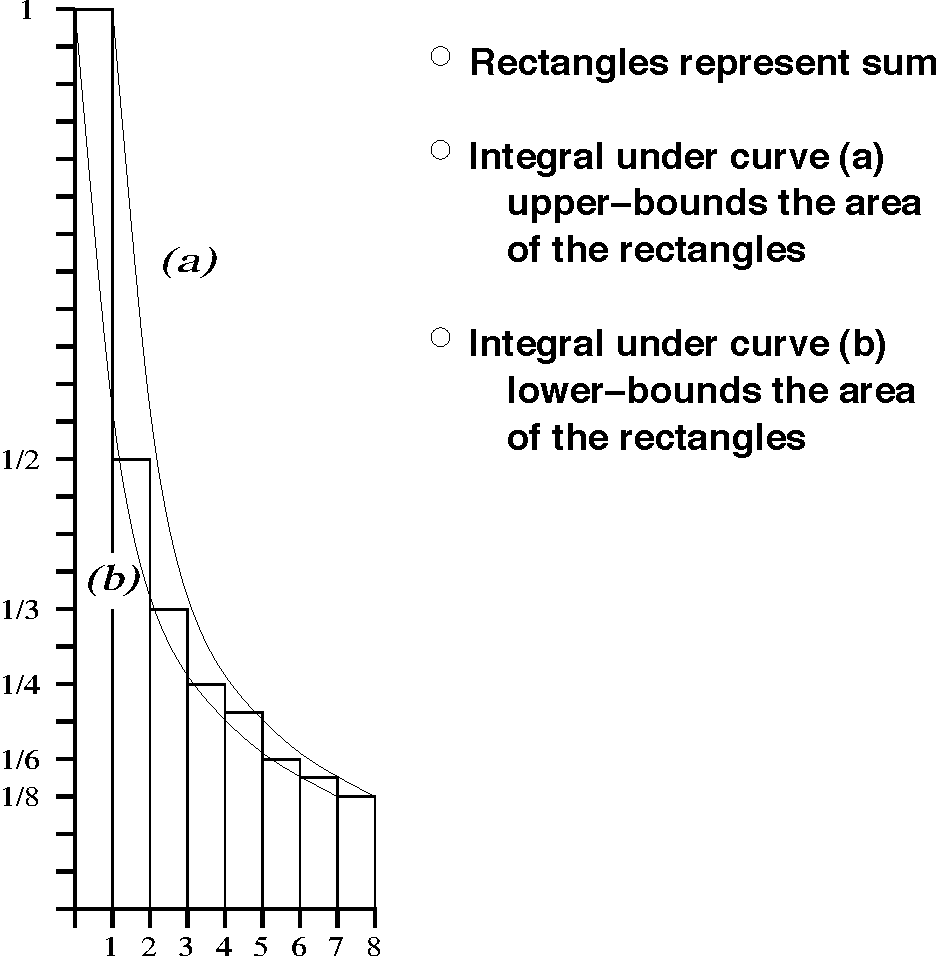
\includegraphics[scale=0.42]{riemann2.pdf}
}
\caption{The summation $S_{(harmonic)}(n) = \sum_{i=1}^n \ 1/i$
  represented by the aggregate area of a sequence of unit-width
  rectangles, and bounded above an below by and ``enveloping'' pair of
  integrals.  The integral that provides the upper bound on the sum
  yields the area under the righthand continuous curve ($a$), namely,
  $\displaystyle \int_1^n \ \frac{1}{x} dx$.  The integral that
  provides the lower bound yields the area under the lefthand
  continuous curve ($b$), namely, $\displaystyle \int_0^{n-1}
  \ \frac{1}{x+1} dx$.}
\label{fig:riemann-harmonic}
\end{figure}

\item
the summation $S_2(n) \eqdef \sum_{i=1}^n \ i^2$ in
Fig.~\ref{fig:riemann-n2}.
\begin{figure}[htb]
\centerline{
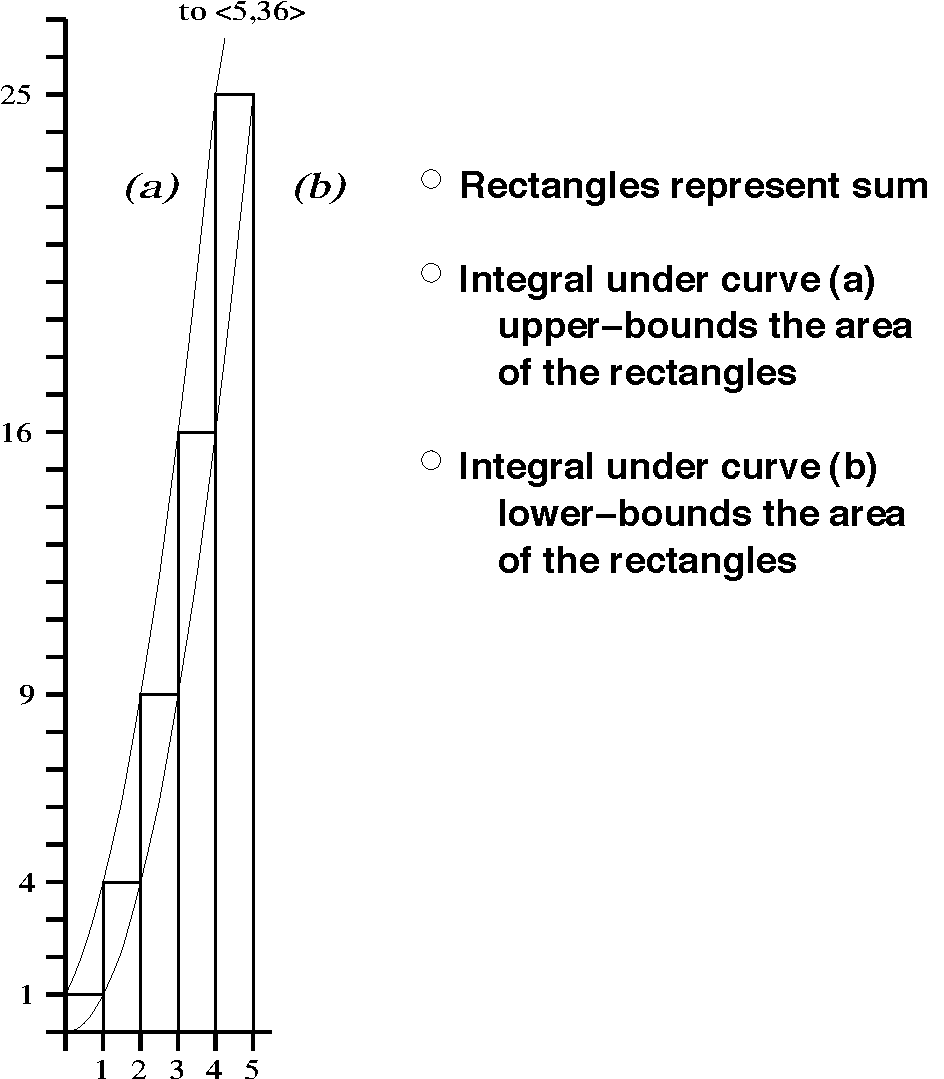
\includegraphics[scale=0.42]{riemann.pdf}
}
\caption{The summation $S_2(n) = \sum_{i=1}^n \ i^2$ represented by
  the aggregate area of a sequence of unit-width rectangles, and
  bounded above an below by and ``enveloping'' pair of integrals.  The
  integral that provides the upper bound on the sum yields the area
  under the lefthand continuous curve ($a$), namely, $\int_0^n
  \ (x+1)^2 dx$.  The integral that provides the lower bound yields
  the area under the righthand continuous curve ($b$), namely,
  $\int_1^n \ x^2 dx$.}
\label{fig:riemann-n2}
\end{figure}
\end{itemizee}
The strategem operates as follows.
\begin{enumerate}
\item
Represent the summands seriatim as abutting unit-width rectangles.  In
Fig.~\ref{fig:riemann-n2}, for instance, these rectangles have heights
$1$, $4$, $9$, $16$, and $25$.  If we were to extend the figure, then
next rectangle would have height $36$.

\item
Construct the continuous curve that will yield (via integration) the
upper bound on the summation so that it passes through the upper
lefthand corners of the unit-width rectangles specified by the
summation.  When constructed appropriately, the area subtended by the
abutting rectangles lie completely under this curve.

\item
Construct the continuous curve that will yield (via integration) the
lower bound on the summation so that it passes through the upper
righthand corners of the unit-width rectangles specified by the
summation.  When constructed appropriately, this curve lies completely
within the area subtended by the abutting rectangles.
\end{enumerate}

\subsubsection{Summing prefixes of the harmonic series.}
TO BE DONE



\subsubsection{Summing successive powers.}
We illustrate the technique of bounding summations via integrals by
focusing on the summations
\[ S_k(n) \ \eqdef \ \sum_{i=1}^n \ i^k, \]
for arbitrary positive integers $k$.  The technique generalizes far
beyond the summations $S_k(n)$, but this single illustration should
give the reader a firm basis from which to extrapolate to more general
summations.

We begin by describing the technique in detail for the summation
$\displaystyle S_2(n) = \sum_{i=1}^n \ i^2$.  We shall then indicate
how to extrapolate from this case to general summations $S_k(n)$.

We obtain our upper bound on $S_2(n)$ by evaluating the integral that
yields the area $\overline{A}_2(n)$ under the lefthand continuous
curve ($a$) in Fig.~\ref{fig:riemann-n2}, namely,
\begin{eqnarray}
\label{eq:upper-integral-x2}
\overline{A}_2(n) \ = \
\int_0^n \ (x+1)^2 dx & = &
  \int_0^n \ x^2 dx \ + \ 2 \int_0^n \ x dx \ + \ \int_0^n \ dx \\
\nonumber
 & = & \frac{1}{3} n^3 \ + n^2 \ + \ n \ + \ O(1).
\end{eqnarray}
We obtain our lower bound on $S_2(n)$ by evaluating the integral that
yields the area $\underline{A}_2(n)$ under the righthand continuous
curve ($b$) in the the figure, namely,
\begin{equation}
\label{eq:lower-integral-x2}
\underline{A}_2(n) \ = \
\int_1^n \ x^2 dx \ = \ \frac{1}{3} n^3 \ + \ O(1).
\end{equation}
Combining these bounds, we finally have the following two-sided bound
on $S_2(n)$.
\begin{equation}
\label{eq:bounds-sum-x2}
\frac{1}{3} n^3 \ + \ O(1)
  \ \ \leq \ \ \sum_{i=1}^n \ i^2
  \ \ \leq \ \ \frac{1}{3} n^3 \ + n^2 \ + \ n \ + \ O(1)
\end{equation}

\medskip

For summations $S_k(n)$ with $k >2$, we follow the roadmap of the case
$k=2$, invoking as a technical tool the following special case of
Newton's {\it Binomial Theorem}.\footnote{The general form of the
  Binomial Theorem expands the polynomial $(x+y)^k$ rather than
  $(x+1)^k$.}

\bigskip

\noindent {\bf The Restricted Binomial Theorem.}
{\em
For all positive integers} $k$, \
$\displaystyle (x+1)^k \ = \
\sum_{i=0}^k \ \ {k \choose i} x^{k-i}$.
\footnote{
As usual, the {\it binomial coefficients} are defined and denoted as
follows.
\[
{k \choose i} \ = \ \frac{k!}{i!(k-i)!} \ = \
\frac{k(k-1)(k-2) \cdots (k-i+1)}{i(i-1)(i-2) \cdots 1}
\]}

The extrapolation from $S_2(n)$ to general $S_k(n)$ begins with the
straightforward exercise of crafting analogues of
Fig.~\ref{fig:riemann-n2} for arbitrary summations $S_k(n)$.
Parallelling the reasoning that led us to the relations
(\ref{eq:upper-integral-x2}) and (\ref{eq:lower-integral-x2}) we
obtain:
\begin{itemize}
\item
an upper bound on summation $S_k(n)$ by evaluating the integral that
yields the area $\overline{A}_k(n)$ under the continuous curve that
passes through the upper lefthand corners of the unit-width rectangles
specified by summation $S_k(n)$.
\begin{eqnarray}
\label{eq:upper-integral-xk}
\overline{A}_k(n) \ = \
\int_0^n \ (x+1)^k dx & = &
\int_0^n \ \left(
\sum_{i=0}^k \ \ {k \choose i} x^{k-i} \right) dx \\
\nonumber
  & = &
\sum_{i=0}^k \ \ \frac{1}{k-i+1} {k \choose i} n^{k-i+1} \ + \ O(1)
\end{eqnarray}
This is a proper upper bound because the region defined by this curve
totally contains the region subtended by the rectangles.

\item
a lower bound on summation $S_k(n)$ by evaluating the integral that
yields the area $\underline{A}_k(n)$ under the continuous curve that
passes through the upper righthand corners of the unit-width
rectangles specified by summation $S_k(n)$.
\begin{equation}
\label{eq:lower-integral-xk}
\underline{A}_k(n) \ = \ 
\int_1^n \ x^k dx \ = \ \frac{1}{k+1} n^{k+1} \ + \ O(1).
\end{equation}
This is a proper lower bound because the region subtended by the
rectangles totally contains the below this curve
\end{itemize}

\noindent
Using this strategy, one finds that for any positive integer $k$,
summation $S_k(n)$ enjoys the following two-sided bound:
\begin{equation}
\label{eq:bounds-sum-xk}
\frac{1}{k+1} n^{k+1} \ + \ O(1)
  \ \ \leq \ \ \sum_{i=1}^n \ i^k
  \ \ \leq \ \ 
\sum_{i=0}^k \ \ \frac{1}{k-i+1} {k \choose i} n^{k-i+1} \ + \ O(1)
\end{equation}
It follows that $S_k(n)$ enjoys the following asymptotic behavior.
\begin{equation}
\label{eq:behavior-sum-xk}
S_k(n) \ = \
\sum_{i=1}^n \ i^k \ \approx \ \frac{1}{k+1} \ n^{k+1}.
\end{equation}

\medskip

We now discuss how to ``expand'' bounds such as
(\ref{eq:bounds-sum-xk}) into explicit expressions for the summations
$S_k(n)$.


\subsection{On Using {\em Undetermined Coefficients} to Obtain Explicit Sums}
\label{sec:undetermined-coefficients}
\index{method of undetermined coefficients}

This section introduces the {\em Method of Undetermined Coefficients},
a tool that can sometimes refine approximations to summations to exact
explicit expressions.  We illustrate the tool on the summations
$S_k(n)$ that we studied in Section~\ref{sec:riemann-bounds}; we use
the tool to convert bounds on the $S_k(n)$, such as
(\ref{eq:behavior-sum-xk}), to explicit expressions for the
summations.

We illustrate the method by deriving explicit expressions for two
rather simple summations: the sum $S_1(n)$ of the first $n$ positive
integers and the sum $S_2(n)$ of the first $n$ perfect squares.

\noindent {\it Expressing $S_1(n)$ explicitly.}
%
Of course, we have already determined $S_1(n)$ in
Section~\ref{sec:arithmetic-series}, by other means.  We provide this
alternative derivation as a gentle introduction to the method of
undetermined coefficients.

\noindent {\bf Proposition.}
{\em For all} $n \in \N$,
\[
S_1(n) \ \eqdef \ \sum_{i=1}^n \ i^2 
 \ = \  1 + 2 + \cdots + n
 \ = \  \frac{1}{2} n^2 \ + \ \frac{1}{2} n
\]

\begin{proof}
We can reason from the case $k=1$ of (\ref{eq:bounds-sum-xk}) that
\[ S_1(n) \ = \ \frac{1}{2} n^2 \ + \ cn \]
for some positive constant $c$, the eponymous {\it undetermined
  coefficient} for this case.  We can discover the value of $c$ by
evaluating $S_1(n)$ at the value $n =1$.  Any value of $n$ will work;
using the {\em smallest} one simplifies our calculation.

Because $S_1(1) = 1$, we
have
\[ S_1(1) \ = \ 1 \ = \ \frac{1}{2} \ + \ c, \]
so that $c = 1/2$; in other words,
\[ S_1(n) \ = \ \frac{1}{2} \left( n^2 + n \right) \ = \ 
\frac{n(n+1)}{2}.
\]
\end{proof}
We verify this expression by induction in
Proposition~\ref{thm:sum-1-to-n-induction}.

\medskip

\noindent {\it Expressing $S_2(n)$ explicitly.}
%
A modestly more complicated undetermined-coefficient calculation
allows us to evaluate the sum $S_2(n)$ of the first $n$ squares.

\noindent {\bf Proposition.}
{\em For all} $n \in \N$,
\begin{equation}
\label{eq:sum-1-to-nsq}
S_2(n) \ \eqdef \ \sum_{i=1}^n \ i^2 
 \ \eqdef \  1 + 4 + \cdots + (n-1)^2 + n^2
 \ = \ \frac{1}{3} n^3 \ + \ \frac{1}{2} n^2 \ + \ \frac{1}{6} n
\end{equation}

$S_2(n)$ is often expressed in a more aesthetic form:
\[ S_2(n) \ = \
\frac{1}{6} n (n+1)(2n+1) \ = \
\frac{2n+1}{3} \cdot {n \choose 2}.
\]

\begin{proof}
We can reason from the case $k=2$ of (\ref{eq:bounds-sum-xk}) that
\begin{equation}
\label{eq:symbolic-cubic}
\sum_{i=0}^n \ k^2 \ = \ \frac{1}{3} n^3 + c_2 n^2 + c_1 n.
\end{equation}
for some positive numbers $c_2$ and $c_1$, the eponymous {\it
  undetermined coefficient} for this case.

We begin our determination of the constants $c_1$ and $c_2$ by
instantiating the polynomial in (\ref{eq:symbolic-cubic}) with the
smallest two values of $n$, namely, $n = 1,2$.  Of course, any two
values will work, but using the {\em smallest} ones simplifies
calculations.  These instantiations leave us with the following pair
of linear equations.
\[
\begin{array}{cccccl}
n=1: & \sum_{i=0}^1 \ k^2
   & = & 1 & = &
1/3 \ + \ c_2 \ + \ c_1 \\
n=2: & \sum_{i=0}^2 \ k^2
   & = & 5 & = &
8/3 \ + \ 4 c_2 \ + \ 2 c_1
\end{array}
\]
By elementary arithmetic, these equations simplify to yield the pair
\[
\begin{array}{ccc}
c_2 \ + \ c_1   & = & 2/3 \\
2 c_2 \ + \ c_1 & = & 7/6
\end{array}
\]
These equations reveal that
\[ 2/3 \ - \ c_2 \ = \ 7/6 \ - \ 2 c_2 \]
so that 
\[ c_2 \ = \ 1/2 \]
which means that
\[ c_1 \ = \ 1/6. \]
We have, thus, derived equation~(\ref{eq:sum-1-to-nsq}).  \qed
\end{proof}

With more (calculational) work, but no new (mathematical) ideas, one
can derive explicit expressions for the sum of the first $n$ $k$th
powers, i.e., the quantity $S^{(k)}_n$, for any positive integer $k$.


\subsection{Validating Approximate Sums via Induction}
\label{sec:Sums-Induction}


We illustrate the proof technique of (Finite) Induction by proving the
correctness of two familiar summation formulas: (1) the sum of the
first $n$ positive integers and (2) the sum of the first $n$ odd
positive integers.


\begin{center}
\label{thm:sum-1-to-n-induction}
For all $n \in \N$,
\begin{eqnarray}
\nonumber
S_n \ \eqdef \ \sum_{i=1}^n \ i
 & \eqdef &
 1 + 2 + \cdots + (n-1) + n \\
\label{eq:sum-first-n}
 & = & {1 \over 2} n (n+1) \\
\nonumber
 & = & {{n+1}  \choose 2}.
\end{eqnarray}
\end{center}

\begin{proof}
For every positive integer $m$, let {\bf P}$(m)$ be the proposition
\[  1 + 2 + \cdot + m \ = \ {{m+1} \choose 2}. \]
Let us proceed according to the standard format of an inductive
argument.

{\bf 1.} Because ${\displaystyle {2 \choose 2}} = 1$, proposition {\bf
  P}$(1)$ is true.

{\bf 2.} Let us assume, for the sake of induction, that proposition
{\bf P}$(m)$ is true for all positive integers strictly smaller than
$n$.  In particular, then, {\bf P}$(n-1)$ is true.

{\bf 3.} Consider now the summation
\[ 1 + 2 + \cdots + (n-1) + n. \]
Because {\bf P}$(n-1)$ is true, we know that
\[ 1 + 2 + \cdots + (n-1) \ = \ {n \choose 2}.  \]
By direct calculation, we see that
\begin{eqnarray*}
{n \choose 2} + n
  & = & \frac{n(n-1)}{2}  \ + \ n \\ 
  & = & \frac{n^2 - n + 2n}{2} \\
  & = & \frac{n^2 + n}{2} \\
  & = & {{n+1} \choose 2}
\end{eqnarray*}

Because $n$ is an arbitrary positive integer, we conclude that
{\bf P}$(n)$ is true whenever
\begin{itemize}
\item
{\bf P}$(1)$ is true
\item
{\em and}
{\bf P}$(m)$ is true for all $m < n$.
\end{itemize}
By the Principle of (Finite) Induction, then, we conclude that {\bf
  P}$(n)$ is true for all $n \in \N^+$.
\qed
\end{proof}

\bigskip

We turn now to our second summation, which asserts that each perfect
square of a positive integer, say, $n^2$, is the sum of the first $n$
odd integers, $1, 3, 5, \ldots, 2n-1$.  This proof complements the
constructive proofs of the same result in
Proposition~\ref{thm:squares-odd-integers-Gauss}.

\begin{center}
\label{thm:squares-odd-integers-induction}
For all $n \in \N^+$,
\[
\sum_{k=1}^n \ (2k-1)
 \ = \ 1 + 3 + 5 + \cdots + (2n-1) \ = \ n^2.
\]
That, is, the $n$th perfect square is the sum of the first $n$ odd
integers.
\end{center}

\noindent {\em Verification.}
%
For every positive integer $m$, let {\bf P}$(m)$ be the proposition
\[ m^2 \ = \ 1 + 3 + 5 + \cdots + 2m-1. \]
Let us proceed according to the standard format of an inductive
argument.

{\bf 1.} Because $1 \cdot 1 = 1$, proposition {\bf P}$(1)$ is true.

{\bf 2.} Let us assume, for the sake of induction, that proposition
{\bf P}$(m)$ is true for all positive integers strictly smaller than
$n$.  In particular, then, {\bf P}$(n-1)$ is true.

{\bf 3.} Consider now the summation
\[ 1 + 3 + 5 + \cdots + 2n-3 + 2n-1 \]
Because {\bf P}$(n-1)$ is true, we know that
\[ 1 + 3 + 5 + \cdots + 2n-3 + 2n-1 \ = \ (n-1)^2 + 2n-1.  \]
By direct calculation, we see that
\[ (n-1)^2 + 2n-1 \ = \ (n^2 -2n +1) + (2n-1) \ = \ n^2. \]
Because $n$ is an arbitrary positive integer, we conclude that
{\bf P}$(n)$ is true whenever
\begin{itemize}
\item
{\bf P}$(1)$ is true
\item
{\em and}
{\bf P}$(m)$ is true for all $m < n$.
\end{itemize}
By the Principle of (Finite) Induction, then, we conclude that {\bf
  P}$(n)$ is true for all $n \in \N^+$.
\qed

\begin{thebibliography}{9}
\bibitem{CLRS}
T.H.~Cormen, C.E.~Leiserson, R.L.~Rivest, C.~Stein (2001):
{\it Introduction to Algorithms (2nd ed.)}.
MIT Press, Cambridge, MA.
\end{thebibliography}

\end{document}
